
\documentclass[afourpaper]{tufte-handout}

\title{Fraktale Bildcodierung}
\author{Jens Ochsenmeier}
\date{}

% bold math
\usepackage{bm}
\usepackage[parfill]{parskip}

\begin{document}

\maketitle% this prints the handout title, author, and date

\begin{abstract}
\noindent
  Inhalt des Vortrags ist \dots
\end{abstract}

\section{Recap --- bisherige Themen}

\subsection{Metrischer Raum}

Ein \emph{metrischer Raum} ist eine Menge \( X \) mit einer reellwertigen Funktion \( X \times X \to \R \). Diese misst den Abstand zwischen zwei Punkten \( x,y \in X \) und muss dazu folgende Axiome erfüllen (\( x,y,z \in X \)):
\begin{enumerate}
  \item \textbf{Symmetrie}: \( d(x,y) = d(y,x) \)
  \item \textbf{Positive Definitheit}: \( 0 \leq d(x,y) \) und \( d(x,y) = 0 \Rightarrow x = y \)
  \item \textbf{Dreiecksungleichung}: \( d(x,z) \leq d(x,y) + d(y,z) \)
\end{enumerate}

Mithilfe von Cauchy-Folgen lassen sich nun \emph{vollständige metrische Räume} konstruieren. Insbesondere brauchen wir \emph{kompakte metrische Räume}, eine Teilmenge der vollständigen metrischen Räume.

\subsection{``Raum der Fraktale''}

Für eine gegebene Menge \( X \) bezeichnen wir zunächst die Menge aller kompakten Teilmengen von \( X \) mit \( \mathcal{H}(X) \). Die leere Menge schließen wir hierbei aus.

Um mit \( \mathcal{H}(X) \) arbeiten zu können definieren wir passende Abstandsbegriffe:
\begin{itemize}
  \item \( d(x,A) = \min\left \{ d(x,a) : a \in A \right \} \) (\( x \in X \), \( A \in \mathcal{H}(X) \)) sei der Abstand zwischen einem Punkt \( x \in X \) und einem Element \( A \) von \( \mathcal{H}(X) \).
  \item \( d(A,B) = \max\left \{ d(x,B) : x \in A \right \} \) sei der Abstand zwischen zwei Mengen in \( \mathcal{H}(X) \).
\end{itemize}

Mithilfe dieser Abstandsbegriffe konstruieren wir die \emph{Hausdorff-Distanz} zwischen zwei Mengen \( A,B \in \mathcal{H}(X) \) durch
\begin{equation*}
  h(A,B) \coloneqq \max\left \{ d(A,B),\ d(B,A) \right \}\text{.}
\end{equation*}
Die Hausdorff-Distanz bildet eine Metrik auf \( \mathcal{H}(X) \).

Wir erhalten den \emph{Raum der Fraktale}
\begin{equation*}
  (\mathcal{H}(X), h)\text{.}
\end{equation*}
Für uns ist --- zumindest vorerst --- jede Teilmenge von \( (\mathcal{H}(X), h) \) ein Fraktal. Weiter kann gezeigt werden, dass folgender zentraler Satz über den Raum der Fraktale gilt:

\begin{theorembox}
  \textbf{Vollständigkeit des Raums der Fraktale} \\
  \vspace{1mm}
  Es gilt
  \begin{align*}
    (X,d) &\text{ ist ein vollständiger metrischer Raum} \\
    \Rightarrow (\mathcal{H}(X), h) &\text{ ist ein vollständiger metrischer Raum.}
  \end{align*}
\end{theorembox}

\subsection{Kontraktionen}

Eine \emph{Kontraktion} ist eine spezielle Abbildung \( \phi: X \to X \), für die ein \( c \in [0,1) \) existiert, sodass
\begin{equation*}
  \forall x,y \in X : d(\phi(x), \phi(y)) \bm{\leq} c * d(x,y)\text{.}
\end{equation*}
\( c \) wird hier als \emph{Kontraktionsfaktor} bezeichnet.
Eine Kontraktion zieht eine Menge ``in sich selbst zusammen'' --- mindestens so stark wie eine zentrische Streckung mit festem Streckungsfaktor \( c < 1 \).

Ein wichtiger Sonderfall einer Kontraktion liegt vor, wenn
\begin{equation*}
  \forall x,y \in X : d(\phi(x), \phi(y)) \bm{=} c * d(x,y)\text{.}
\end{equation*}
Eine solche Kontraktion wird \emph{Ähnlichkeitsabbildung} genannt, \( c \) heißt hier \emph{Kontraktionsverhältnis}.

\subsection{Iterierte Funktionensysteme (IFS)}

Ein \emph{iteriertes Funktionensystem} (IFS) ist Familie endlich vieler Kontraktionen auf einem vollständigen metrischen Raum, hier sei \( (X,d) \) ein solcher Raum und \( \left \{ \Phi_1, \dots, \Phi_n \right \} \) eine solche Familie.

Der \emph{Kontraktionskoeffizient} eines solchen IFS ist der größte Kontraktionsfaktor seiner Kontraktionen:
\begin{equation*}
  c = \max\left \{ c_1, \dots,c_n \right \} \quad \text{(\( c_i \coloneqq \) Kontraktionsfaktor von \( \Phi_i \))}
\end{equation*}

Erhält man durch Vereinigung der Bilder der Kontraktionen von einer festen Teilmenge \( C \subset X \) wieder \( C \), so ist C der \emph{Attraktor} dieses IFS.\@ Formal:
\begin{equation*}
  C = \bigcup_{i=1}^n \Phi_i(C)\text{.}
\end{equation*}

\section{(Affine) Transformationen}

Aus den Vorlesungen über Lineare Algebra sind lineare Transformationen bekannt. Sie bilden Geraden auf Geraden ab und fixieren den Ursprung. Dargestellt werden können sie durch die Multiplikation eines Vektors mit einer Matrix:
\begin{equation*}
  t: \R^2 \ni \begin{pmatrix}
    x \\ y
  \end{pmatrix} \mapsto \begin{pmatrix}
    a & b \\ c & d
  \end{pmatrix} \begin{pmatrix}
    x \\ y
  \end{pmatrix} \in \R^2
\end{equation*}

Eine (2-dimensionale) \emph{affine Transformation} \( w : \R^2 \to \R^2 \) ist eine Abbildung, die durch
\begin{equation*}
  w(x_1,x_2) = \begin{pmatrix}
    ax_1 + bx_2 + e \\\ cx_1 + dx_2 + f
  \end{pmatrix}
\end{equation*}
für feste \( a,b,c,d,e,f \in \R \) beschrieben werden kann. Eine affine Transformation setzt sich also aus einer linearen Transformation und einer Translation zusammen.

Eine praktische und übliche Notation ist
\begin{equation*}
  w(x) = Ax + t \quad \text{mit} \quad x = \begin{pmatrix}
    x_1 \\ x_2
  \end{pmatrix},\ A = \begin{pmatrix}
    a & b \\ c & d
  \end{pmatrix},\ t = \begin{pmatrix}
    e \\ f
  \end{pmatrix}\text{.}
\end{equation*}

\subsection{Konstruktion einer affinen Transformation}

Sind eine Menge und eine affin transformierte Kopie dieser gegeben, so kann eine passende affine Transformation, die die Menge auf ihre Kopie abbildet, konstruiert werden, indem drei Punkte der Menge und jeweils die dazugehörige Kopie ermittelt werden.

Seien \( (x_1, x_2) \), \( (y_1, y_2) \), \( (z_1, z_2) \) solche Punkte in der Menge und \( (\widetilde{x}_1, \widetilde{x}_2) \), \( (\widetilde{y}_1, \widetilde{y}_2) \), \( (\widetilde{z}_1, \widetilde{z}_2) \) die zugehörigen Punkte in der Kopie.

Daraufhin lassen sich folgende Gleichungen lösen:
\begin{align*}
  \begin{pmatrix}
    x_1 \\ x_2
  \end{pmatrix} \begin{pmatrix}
    a & b \\ c & d
  \end{pmatrix} + \begin{pmatrix}
    e \\ f
  \end{pmatrix} &= \begin{pmatrix}
    \widetilde{x}_1 \\ \widetilde{x}_2
  \end{pmatrix} \\
  \begin{pmatrix}
    y_1 \\ y_2
  \end{pmatrix} \begin{pmatrix}
    a & b \\ c & d
  \end{pmatrix} + \begin{pmatrix}
    e \\ f
  \end{pmatrix} &= \begin{pmatrix}
    \widetilde{y}_1 \\ \widetilde{y}_2
  \end{pmatrix} \\
  \begin{pmatrix}
    z_1 \\ z_2
  \end{pmatrix} \begin{pmatrix}
    a & b \\ c & d
  \end{pmatrix} + \begin{pmatrix}
    e \\ f
  \end{pmatrix} &= \begin{pmatrix}
    \widetilde{z}_1 \\ \widetilde{z}_2
  \end{pmatrix}
\end{align*}

So lassen sich die 6 Parameter einer zugehörigen affinen Transformation bestimmen.


\section{Collage-Theorem}

\section{Page Layout}\label{sec:page-layout}
\subsection{Headings}\label{sec:headings}
This style provides \textsc{a}- and \textsc{b}-heads (that is,
\Verb|\section| and \Verb|\subsection|), demonstrated above.

The Tufte-\LaTeX\ classes will emit an error if you try to use
\linebreak\Verb|\subsubsection| and smaller headings.

% let's start a new thought -- a new section
\newthought{In his later books},\cite{Tufte2006} Tufte
starts each section with a bit of vertical space, a non-indented paragraph,
and sets the first few words of the sentence in \textsc{small caps}.  To
accomplish this using this style, use the \Verb|\newthought| command:  
\begin{docspec}
  \doccmd{newthought\{In his later books\}, Tufte starts\ldots}
\end{docspec}

\subsection{Sidenotes}\label{sec:sidenotes}
One of the most prominent and distinctive features of this style is the
extensive use of sidenotes.  There is a wide margin to provide ample room
for sidenotes and small figures.  Any \Verb|\footnote|s will automatically
be converted to sidenotes.\footnote{This is a sidenote that was entered
using the \texttt{\textbackslash footnote} command.}  If you'd like to place ancillary
information in the margin without the sidenote mark (the superscript
number), you can use the \Verb|\marginnote| command.\marginnote{This is a
margin note.  Notice that there isn't a number preceding the note, and
there is no number in the main text where this note was written.}

The specification of the \Verb|\sidenote| command is:
\begin{docspec}
  \doccmd{sidenote[\docopt{number}][\docopt{offset}]\{\docarg{Sidenote text.}\}}
\end{docspec}

Both the \docopt{number} and \docopt{offset} arguments are optional.  If you
provide a \docopt{number} argument, then that number will be used as the
sidenote number.  It will change of the number of the current sidenote only and
will not affect the numbering sequence of subsequent sidenotes.

Sometimes a sidenote may run over the top of other text or graphics in the
margin space.  If this happens, you can adjust the vertical position of the
sidenote by providing a dimension in the \docopt{offset} argument.  Some
examples of valid dimensions are:
\begin{docspec}
  \ttfamily 1.0in \qquad 2.54cm \qquad 254mm \qquad 6\Verb|\baselineskip|
\end{docspec}
If the dimension is positive it will push the sidenote down the page; if the
dimension is negative, it will move the sidenote up the page.

While both the \docopt{number} and \docopt{offset} arguments are optional, they
must be provided in order.  To adjust the vertical position of the sidenote
while leaving the sidenote number alone, use the following syntax:
\begin{docspec}
  \doccmd{sidenote[][\docopt{offset}]\{\docarg{Sidenote text.}\}}
\end{docspec}
The empty brackets tell the \Verb|\sidenote| command to use the default
sidenote number.

If you \emph{only} want to change the sidenote number, however, you may
completely omit the \docopt{offset} argument:
\begin{docspec}
  \doccmd{sidenote[\docopt{number}]\{\docarg{Sidenote text.}\}}
\end{docspec}

The \Verb|\marginnote| command has a similar \docarg{offset} argument:
\begin{docspec}
  \doccmd{marginnote[\docopt{offset}]\{\docarg{Margin note text.}\}}
\end{docspec}

\subsection{References}
References are placed alongside their citations as sidenotes,
as well.  This can be accomplished using the normal \Verb|\cite|
command.\sidenote{The first paragraph of this document includes a citation.}

The complete list of references may also be printed automatically by using
the \Verb|\bibliography| command.  (See the end of this document for an
example.)  If you do not want to print a bibliography at the end of your
document, use the \Verb|\nobibliography| command in its place.  

To enter multiple citations at one location,\cite{Tufte2006,Tufte1990} you can
provide a list of keys separated by commas and the same optional vertical
offset argument: \Verb|\cite{Tufte2006,Tufte1990}|.  
\begin{docspec}
  \doccmd{cite[\docopt{offset}]\{\docarg{bibkey1,bibkey2,\ldots}\}}
\end{docspec}

\section{Figures and Tables}\label{sec:figures-and-tables}
Images and graphics play an integral role in Tufte's work.
In addition to the standard \docenv{figure} and \docenv{tabular} environments,
this style provides special figure and table environments for full-width
floats.

Full page--width figures and tables may be placed in \docenv{figure*} or
\docenv{table*} environments.  To place figures or tables in the margin,
use the \docenv{marginfigure} or \docenv{margintable} environments as follows
(see figure~\ref{fig:marginfig}):

\begin{marginfigure}%
  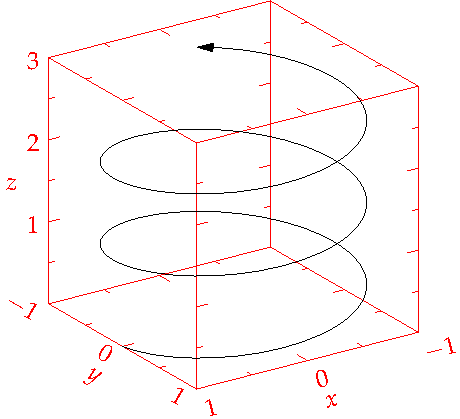
\includegraphics[width=\linewidth]{helix}
  \caption{This is a margin figure.  The helix is defined by 
    $x = \cos(2\pi z)$, $y = \sin(2\pi z)$, and $z = [0, 2.7]$.  The figure was
    drawn using Asymptote (\url{http://asymptote.sf.net/}).}
  \label{fig:marginfig}
\end{marginfigure}
\begin{Verbatim}
\begin{marginfigure}
  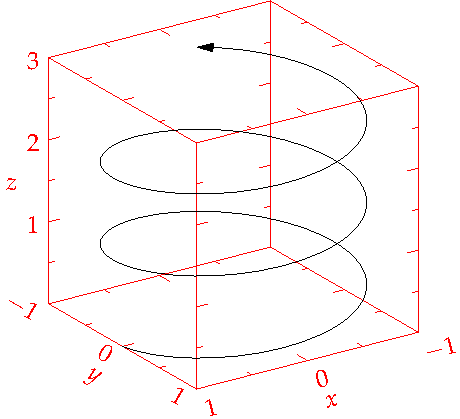
\includegraphics{helix}
  \caption{This is a margin figure.}
\end{marginfigure}
\end{Verbatim}

The \docenv{marginfigure} and \docenv{margintable} environments accept an optional parameter \docopt{offset} that adjusts the vertical position of the figure or table.  See the ``\nameref{sec:sidenotes}'' section above for examples.  The specifications are:
\begin{docspec}
  \doccmd{begin\{marginfigure\}[\docopt{offset}]}\\
  \qquad\ldots\\
  \doccmd{end\{marginfigure\}}\\
  \mbox{}\\
  \doccmd{begin\{margintable\}[\docopt{offset}]}\\
  \qquad\ldots\\
  \doccmd{end\{margintable\}}\\
\end{docspec}

Figure~\ref{fig:fullfig} is an example of the \Verb|figure*|
environment and figure~\ref{fig:textfig} is an example of the normal
\Verb|figure| environment.

\begin{figure*}[h]
  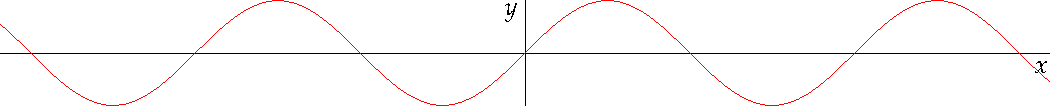
\includegraphics[width=\linewidth]{sine.pdf}%
  \caption{This graph shows $y = \sin x$ from about $x = [-10, 10]$.
  \emph{Notice that this figure takes up the full page width.}}%
  \label{fig:fullfig}%
\end{figure*}

\begin{figure}
  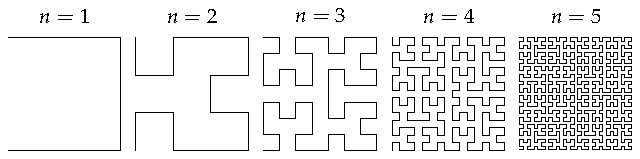
\includegraphics{hilbertcurves.pdf}
%  \checkparity This is an \pageparity\ page.%
  \caption{Hilbert curves of various degrees $n$.
  \emph{Notice that this figure only takes up the main textblock width.}}
  \label{fig:textfig}
  %\zsavepos{pos:textfig}
  \setfloatalignment{b}
\end{figure}

Table~\ref{tab:normaltab} shows table created with the \docpkg{booktabs}
package.  Notice the lack of vertical rules---they serve only to clutter
the table's data.

\begin{table}[ht]
  \centering
  \fontfamily{ppl}\selectfont
  \begin{tabular}{ll}
    \toprule
    Margin & Length \\
    \midrule
    Paper width & \unit[8\nicefrac{1}{2}]{inches} \\
    Paper height & \unit[11]{inches} \\
    Textblock width & \unit[6\nicefrac{1}{2}]{inches} \\
    Textblock/sidenote gutter & \unit[\nicefrac{3}{8}]{inches} \\
    Sidenote width & \unit[2]{inches} \\
    \bottomrule
  \end{tabular}
  \caption{Here are the dimensions of the various margins used in the Tufte-handout class.}
  \label{tab:normaltab}
  %\zsavepos{pos:normaltab}
\end{table}

\section{Full-width text blocks}

In addition to the new float types, there is a \docenv{fullwidth}
environment that stretches across the main text block and the sidenotes
area.

\begin{Verbatim}
\begin{fullwidth}
Lorem ipsum dolor sit amet...
\end{fullwidth}
\end{Verbatim}

\begin{fullwidth}
\small\itshape\lipsum[1]
\end{fullwidth}

\section{Typography}\label{sec:typography}

\subsection{Typefaces}\label{sec:typefaces}
If the Palatino, \textsf{Helvetica}, and \texttt{Bera Mono} typefaces are installed, this style
will use them automatically.  Otherwise, we'll fall back on the Computer Modern
typefaces.

\subsection{Letterspacing}\label{sec:letterspacing}
This document class includes two new commands and some improvements on
existing commands for letterspacing.

When setting strings of the
letter\-spacing---that is, the spacing between the letters---should be
increased slightly.\cite{Bringhurst2005}  The \Verb|\allcaps| command has proper letterspacing for
strings of   These commands
will also automatically convert the case of the text to upper- or
lowercase, respectively.

The \Verb|\textsc| command has also been redefined to include
letterspacing.  The case of the \Verb|\textsc| argument is left as is,
however.  This allows one to use both uppercase and lowercase letters:
\textsc{The Initial Letters Of The Words In This Sentence Are Capitalized.}



\section{Installation}\label{sec:installation}
To install the Tufte-\LaTeX\ classes, simply drop the
following files into the same directory as your \texttt{.tex}
file:
\begin{quote}
  \ttfamily
  tufte-book.cls\\
  tufte-common.def\\
  tufte-handout.cls\\
  tufte.bst
\end{quote}

% TODO add instructions for installing it globally



\section{More Documentation}\label{sec:more-doc}
For more documentation on the Tufte-\LaTeX{} document classes (including commands not
mentioned in this handout), please see the sample book.

\section{Support}\label{sec:support}

The website for the Tufte-\LaTeX\ packages is located at
\url{https://github.com/Tufte-LaTeX/tufte-latex}.  On our website, you'll find
links to our repository, mailing lists, bug tracker, and documentation.

\bibliography{sample-handout}
\bibliographystyle{plainnat}



\end{document}
